% !TEX root = ../../SPP_IoTjournal.tex
\subsection{Results \label{sec:bayArea_simResults}}
The trajectory planning for the vehicles is done using RTT algorithm, similar to that in Section \ref{sec:city_simResults}. The resulting trajectories of vehicles are shown in Figure \ref{fig:bayArea_d11sep5}. Once again, the vehicles remain clear of all other vehicles and reach their respective destinations. Given the relative separation between the scheduled times of arrival, the trajectories are predominately \textit{time-separated}, with roughly two lanes for each pair of cities (one for going from city A to city B and another for from city B to city A). A high-density of vehicles is achieved in the center since the 4 paths are intersecting in the center (Richmond-Oakland, Oakland-Richmond, Berkeley-San Francisco, San Francisco-Berkeley), but the SPP algorithm ensures safety despite this high-density, as shown in the zoomed-in version of center at an intermediate time when a large number of vehicles are passing through the central region (Figure \ref{fig:bayArea_d11sep5_zoomed}).  
%
\begin{figure*}[!htb]
 \centering
\begin{subfigure}{0.5\textwidth}
  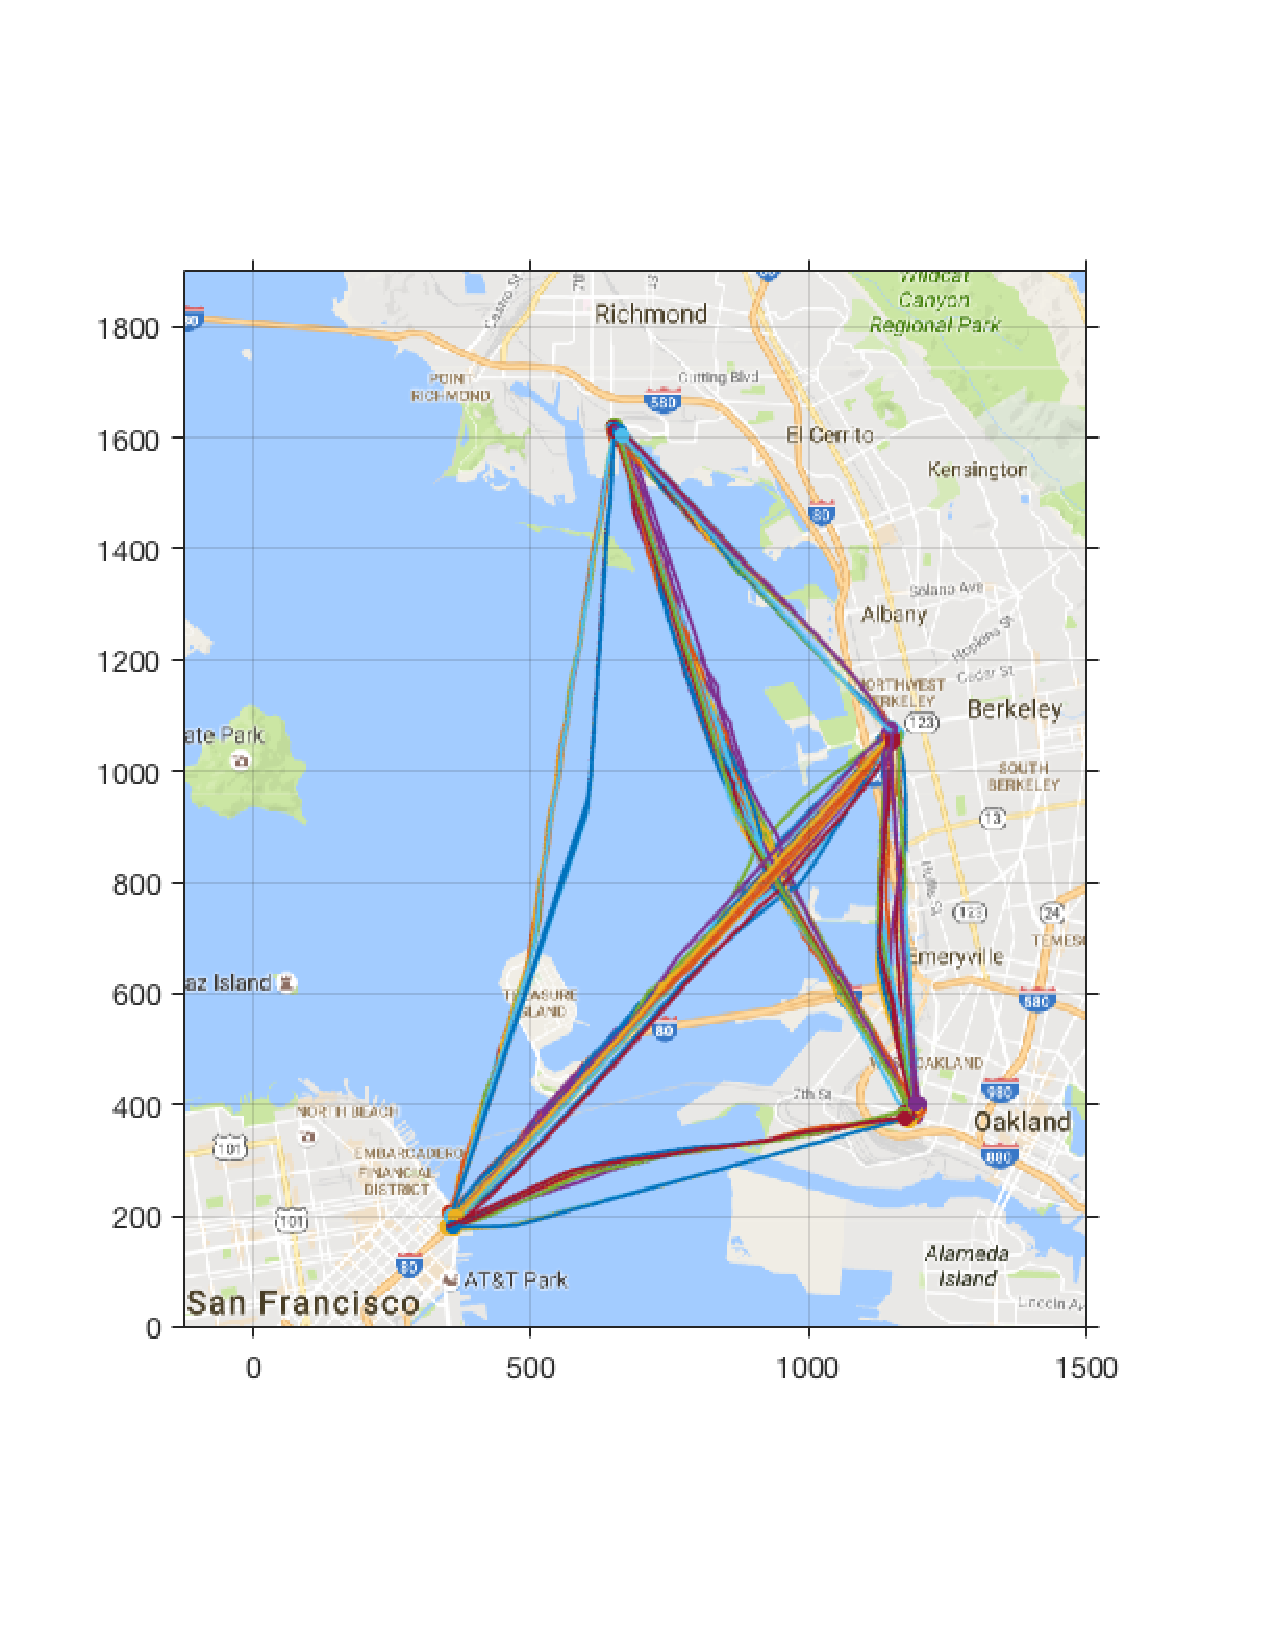
\includegraphics[width=\columnwidth]{figs/bayArea_d11sep5}
  \subcaption{}
  \label{fig:bayArea_d11sep5}
\end{subfigure}%
\begin{subfigure}{0.5\textwidth}
  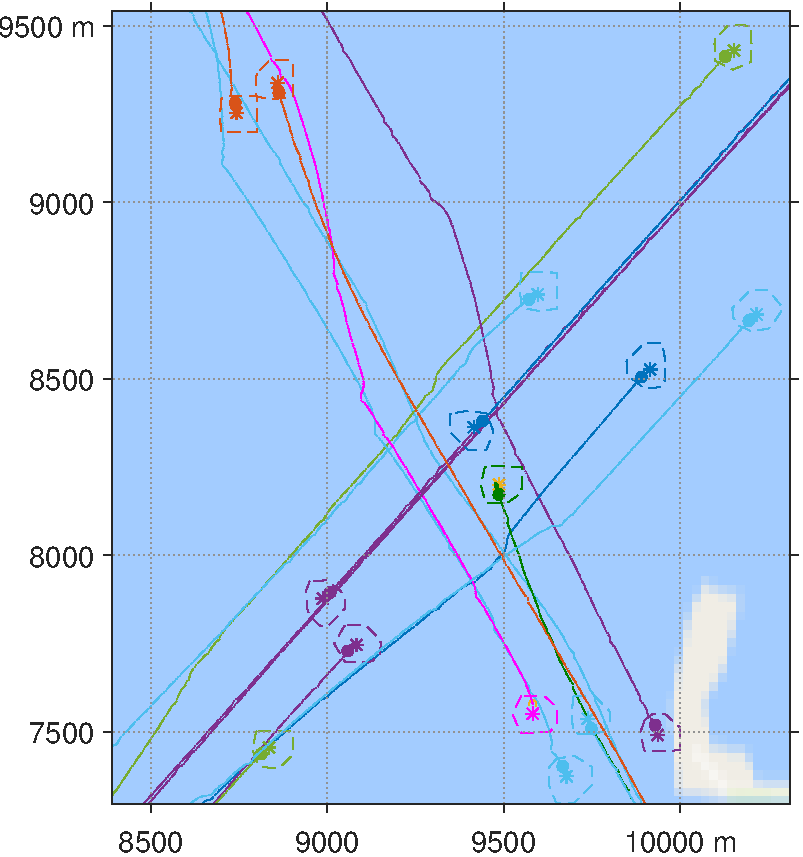
\includegraphics[width=\columnwidth]{figs/bayArea_d11sep5_zoomed}
  \subcaption{}
  \label{fig:bayArea_d11sep5_zoomed}
\end{subfigure}%
  \caption{(a) Trajectories obtained from the SPP algorithm for the multi-city simulation with $d_r = 11m/s$, $\sta_i = 5(i-1)$. (b) Zoomed-in version of the central area. A high density of vehicles is achieved at the center because of the intersection of several trajectories; however, the SPP algorithm still ensures that vehicles do not enter each other's danger zones and reach their destinations.} 
  \label{fig:bayArea_d11sep5_all}
\end{figure*}

Finally, we simulate the system for the case where $\sta_i = 0 ~\forall i$. As evident from Figure \ref{fig:bayArea_d11sep0}, we get multiple lanes between each pair of cities in this case and trajectories become predominately state-separated, as we expect based on the discussion in Section \ref{sec:city_distbEffect}.
\begin{figure}[t]
  \centering
  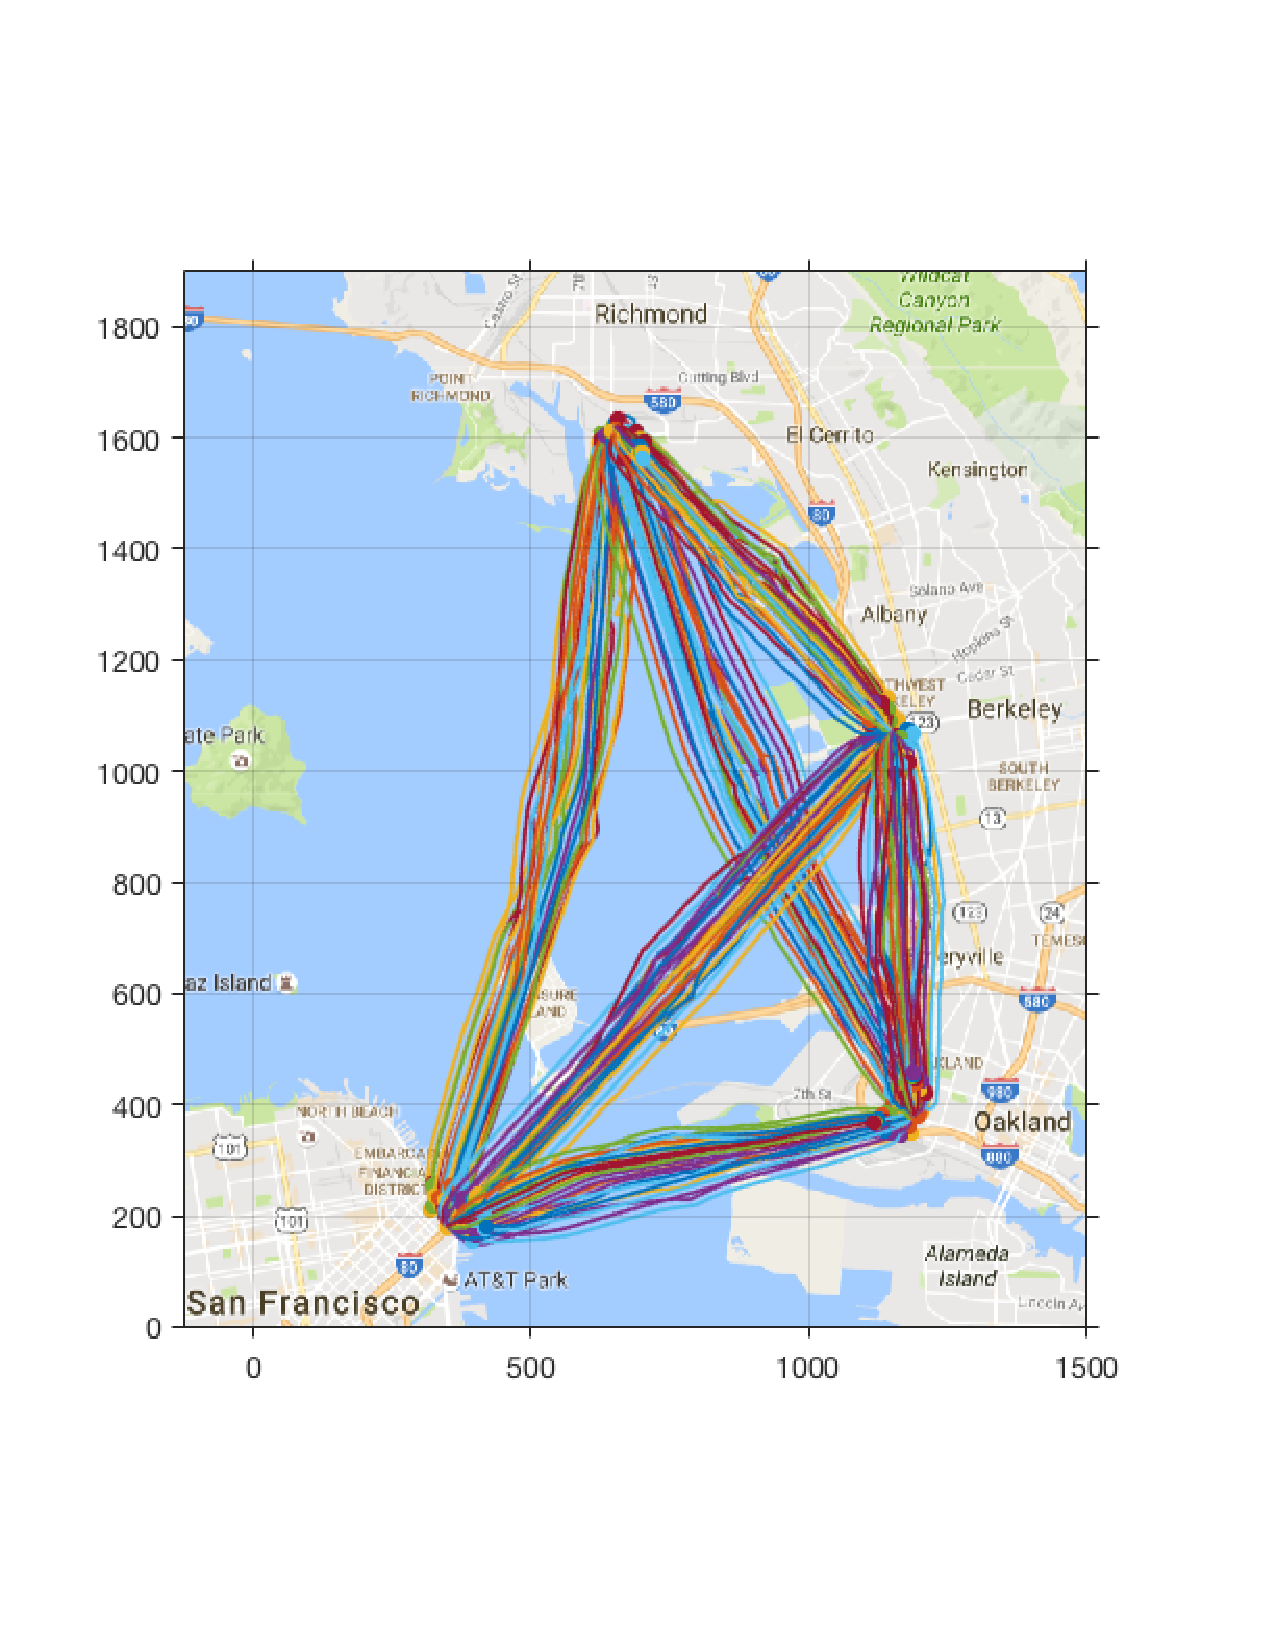
\includegraphics[width=\columnwidth]{figs/bayArea_d11sep0}
  \caption{Vehicle trajectories for $d_r = 11m/s$, $\sta_i = 0$. Since different vehicles have same scheduled times of arrival, a multiple-lane behavior is observed between every pair of cities.} 
  \label{fig:bayArea_d11sep0}
\end{figure}

The average trajectory computation time per vehicle is \SBnote{$XYZ$s} per vehicle on a \SBnote{$Blah Blah$} computing machine. Once again all the computation is done offline and only a lookup table query is required in real-time, which can be performed very efficiently. This simulation illustrates the scalability and the potential of deploying the SPP algorithm for provably safe path planning for large multi-vehicle systems.